
\section{Models}
\noindent
We consider the travel time and travel methods, a total of 26 kinds of programs are proposed, that is, two kinds of travel patterns and thirteen kinds of travel time permutations and combinations. According to our hypothesis, the maximum daily drifting tour time is 8, which is determined by inequality:

\begin{equation}
\left\{ {\begin{array}{*{20}{c}}
	{\frac{S}{{{v_1} \times 8}} \le {T_1}}\\
	{\frac{S}{{{v_2} \times 8}} \le {T_2}}
	\end{array}} \right. \label{aa1}
\end{equation}
%about this eqref \eqref{aa1}\\

We can calculate that for rafts and motorboats, the number of drifting days satisfies ${T_1} \ge 7{T_2} \ge 6$ ,respectively. Therefore, we will exclude the option of including oar-raft and six-day modes of transport, leaving 25 travel options, followed by ${p_1},{p_2},{p_3}...{p_{25}}$ , The specific content of the program is shown in Table \ref{tab:OneSymbols} \ref{tab:Symbol}.
%The minimum number of drifting days for a dinghy can be calculated as 1, so the rubber dinghy and 6-day travel patterns are excluded. There are 25 kinds of travel plans left, followed by 2, and the details of the scheme are shown in Table \ref{tab:Symbols} \ref{tab:Symbol}

\begin{table}[H]
	\centering
	\caption{\label{tab:OneSymbols}Travel programme}
	\begin{tabular}{c c c c c c c r }
		\Xhline{1.2pt}
		Travel days/days  & 6  & 7 & 8 & 9 & 10 & 11 & 12 \\
		\midrule
		Rubber &   & ${p_1}$ & ${p_2}$ & ${p_3}$ & ${p_4}$ & ${p_5}$ & ${p_6}$ \\
		Motorboat &  ${p_{13}}$ & ${p_{14}}$ & ${p_{15}}$ & ${p_{16}}$ & ${p_{17}}$ & ${p_{18}}$ & ${p_{19}}$ \\
		\Xhline{1.2pt} & 
	\end{tabular}
\end{table}

\begin{table}[H]
	\centering
	\caption{\label{tab:Symbol}Travel programme}
	\begin{tabular}{c c c c c c r }
	\Xhline{1.2pt}
	Travel days/days  & 13  & 14 & 15 & 16 & 17 & 18 \\
	\midrule
	Rubber & ${p_7}$ & ${p_7}$ & ${p_9}$ & ${p_{10}}$ & ${p_{11}}$ & ${p_{12}}$ \\
	Motorboat &  ${p_{20}}$ & ${p_{21}}$ & ${p_{22}}$ & ${p_{23}}$ & ${p_{24}}$ & ${p_{25}}$ \\
	\Xhline{1.2pt} & 
\end{tabular}
\end{table}
As shown in Table \ref{tab:OneSymbols} \ref{tab:Symbol},we fixed the travel options into 25 categories, that is, the river management companies have a total of 25 travel plans for tourists to choose from.

%插流程图
\par To show our optimization model more clearly and clearly, we sketch the modeling flowchart as follows:
\begin{figure}[H]
	\centering
	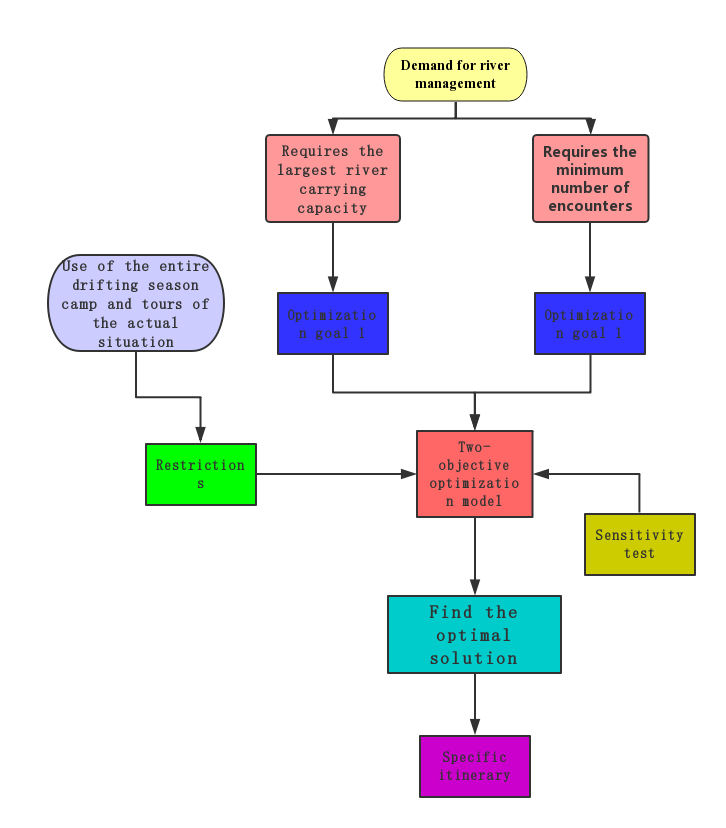
\includegraphics[width=0.7\linewidth]{figures/flowchart}
	\caption{The modeling flowchart}
	\label{fig:flowchart}
\end{figure}

  
%about this eqref \eqref{aa1}
\subsection{Optimize the use of camping sites}
\label{subsection:5.1subsection}
\noindent 
Firstly, we define the carrying capacity of a river as the number of tours a river can accommodate each year. Secondly, we set the number of campsites as fixed value. In order to maximize the utilization of campsites, we use mathematical programming model to ensure the maximum number of camps to use as the goal. In addition, our model is required to ensure that the tour groups do their best during drifting may not touch each other.Considering both the two we create a dual-objective optimization model.
\par In order to facilitate the establishment of our model will define and explain some of the concepts below.

\subsubsection{Some necessary preparation}
\begin{enumerate}
	\item[1)]Unit camp matrix 
	\par The unit camp matrix $U_i^k$ represents the case where each campground is utilized when the travel plan ${p_i}$ is executed for the $k$ time, which is a matrix of ${n_i} \times Y$, ${n_i}$ indicates the travel days corresponding to the plan ${p_i}$, and the elements in $U_i^k$ are defined as $u_{mn}^i$ follows:
	\begin{equation}
		u_{mn}^i = \left\{ {\begin{array}{*{20}{c}}
			{\rm{1}}&{{\rm{The\; n-th\; camp\ was\ occupied\ on\ the\; m-th\; night}}}\\
			{\rm{0}}&{{\rm{otherwise}}}
			\end{array}} \right.\label{aa1}
	\end{equation}
	
	\item[2)]Camping matrix
		\par The camping matrices indicate occupancy of campsites when the travel plan ${p_i}$ is executed throughout the drifting season, and we add up the matrices $U_i^k$ ,on the basis of which the zero matrices complement corresponding to night when the travel plan is not implemented and are expanded to matrices The elements of the matrices in the matrix are defined as follows:
		\begin{equation}
			c_{mn}^i = \left\{ {\begin{array}{*{20}{c}}
			{\rm{1}}&{{\rm{The\; n-th\; camp\ was\ occupied\ on\ the\; m-th\; night}}}\\
			{\rm{0}}&{{\rm{otherwise}}}
			\end{array}} \right.\label{aa1}
		\end{equation}
		According to the definition of camping matrices and camping matrices we can see:
		\begin{equation}
			c_{mn}^i = \left\{ {\begin{array}{*{20}{c}}
			{u_{mn}^i}&{{\rm{When\ travel\ plan\;  }}{p_i}\;{\rm{ is\ executed}}}\\
			{\rm{0}}&{{\rm{otherwise}}}
			\end{array}} \right.\label{aa1}
		\end{equation}
		In this section we make some necessary preparations for the following model establishment, which is very helpful for us to establish a good model.
	
	\item[3)]Total camp camp matrix
	\par The total camp matrix $A$ represents the utilization of the entire drifting season camp, which is the sum of the matrices ${C_i}(i = 1,2,3,...,25)$ and whose element ${a_{mn}}$ is defined as follows:
	\begin{equation}
		{a_{mn}} = \left\{ {\begin{array}{*{20}{c}}
			{\rm{1}}&{{\rm{The\; n-th\; camp\ was\ occupied\ on\ the\; m-th\; night}}}\\
			{\rm{0}}&{{\rm{otherwise}}}
			\end{array}} \right.\label{aa1}
	\end{equation}
	It is clear from its definition of ${a_{mn}} = \sum\limits_{i = 1}^{25} {c_{mn}^i} $.
	In this section, we make some necessary preparations for the following model establishment, which is very helpful for us to establish a good model.
\end{enumerate}

\subsubsection{Utilization of camping sites}
%\label{subsection:5.2subsection}
\noindent
As we explained in the Problem Analysis section, we use the number of campsites as the goal of optimization. According to the definition of preparation part can get the first optimization objective function, as follows:
	\begin{equation}
	\max \sum\limits_{m = 1}^{179} {\sum\limits_{n = 1}^Y {{a_{mn}}} }\label{aa1}
	\end{equation}
In the following section we will determine the constraints of the model.
\par For unit camping matrices, each tour group occupies only one camp overnight and thus:
	\begin{equation}
	\sum\limits_{n = 1}^Y {u_{mn}^i} {\rm{ = }}1\label{aa1}
	\end{equation}
On request, the same camp can only accommodate one tour group on the same night, so there:
	\begin{equation}
	\sum\limits_{i = 1}^{25} {c_{mn}^i}  \le 1\label{aa1}
	\end{equation}
And we take that how many the camping site could accommodate the total number of tours per night into count,we have:
	\begin{equation}
	\sum\limits_{i = 1}^{25} {\sum\limits_{n = 1}^Y {c_{mn}^i \le Y} }\label{aa1}
	\end{equation}	
\par At the same time, we consider that any tour group is free to choose the daily trip, but according to our assumption that the maximum drifting time can not exceed 8h, so it has the following restrictions on the itinerary:
	\begin{equation}
	\left\{ {\begin{array}{*{20}{c}}
		{0 < t_j^iv \le 8v,\;{\rm{the\ first\ day\ of\  the\ travel\ plan\ }}{p_i}}\\
		\\
		{0 < \frac{S}{{Y + 1}}(q - p) \le 8v,\;{\rm{Rest}}}\\
		\\
		{{\rm{   }}0 < S - \sum\limits_{j = 1}^{{n_i}} {vt_j^i \le 8v,\;{\rm{The\ last\ day\ of\ the\ travel\ plan\ }}{p_i}} }
		\end{array}} \right.\label{aa1}
	\end{equation}
There $v = {v_1},{v_2}$ ,we let $t_j^i$ indicate that the time when the tour group carrying out the travel plan ${p_i}$ drift on the jth day, $q,p$  respectively indicate the number of campsites where the same group will be camping on two adjacent nights. From this we can get the following constraints:
	\begin{equation}
	\left\{ {\begin{array}{*{20}{c}}
		{c_{mp}^i = 1}\\
		\\
		{c_{(m + 1)q}^i = 1}
		\end{array}} \right.{\rm{        }}i = 1,2,...,25\label{aa1}
	\end{equation}
	\par The above formula shows that the distance between two campsites for any two consecutive nights can not exceed the maximum daily drifting distance.

\subsection{Reduce the number of contacts}
\label{subsection:5.2subsection}
First, we clarify the specific meaning of contacts in the subject, that is, which situations can be called contacts. According to the subject, we define the same point where we reach the river at the same time as the rafting process. Second, we define the departure date matrix for the tour within 180 days. Its element $d_j^{}$ is defined as follows: 
	\begin{equation}
	{d_j} = J + {n_i}\label{aa1}
	\end{equation}
	Where $J$ indicates that the launch date of the tour group choosing travel plan ${p_i}$ is the $j$ th day of draft season, ${n_i}$ is the number of nights camping on a travel plan ${p_i}$.
	\par When the two tours meet, according to the definition of encounter we may have:
	\begin{equation}
	{\rm{   }}\left\{ {\begin{array}{*{20}{c}}
		{v\sum\limits_{j = 1}^\beta  {t_{ij}^{} = v\sum\limits_{j = 1}^{{\beta ^ * }} {t_{ij}^ * } } }&{}\\
		\\
		{{J_{}} + \sum\limits_{j = 1}^\beta  {t_{ij}^{}}  = {J^ * } + \sum\limits_{j = 1}^{{\beta ^ * }} {t_{ij}^ * } }&{}
		\end{array}} \right.0 < \beta {\beta ^ * } \le {n_i}\label{aa1}
	\end{equation}
	Where $v = {v_{1,}}{v_2}$, and $t_{ij}^{}$, $t_{ij}^ * $represents drifting the time of a tour on $j$-th day.
	\par Defined $\lambda $ as the number of contacts, whose expression is as follows:
	\begin{equation}
	\lambda  = \left\{ {\begin{array}{*{20}{c}}
		{\lambda  +  + }&{{\rm{  \quad    (14)\; Form\ set\ up}}}\\
		\lambda &{{\rm{otherwise}}}
		\end{array}} \right.\label{aa1}
	\end{equation}
	\par So we get the second optimization Goal $\lambda $:
	\begin{equation}
	\min \left\{ \lambda  \right\}\label{aa1}
	\end{equation}
	
\subsection{Itinerary Plan}
\noindent Below we use the \textbf{two-objective optimization model} built in Sections \ref{subsection:5.1subsection} and \ref  {subsection:5.2subsection} to find out the best travel arrangements under the premise of ensuring the most frequent use and the minimum number of contacts in the campsite, and the management can provide the tourists with our scheme select. To ease the solution, we weaken the weaker target in the dual-objective into a constraint, and by adjusting it we can relax or tighten the constraint. Finally, our mathematical model is as follows:
	\begin{equation}
	\max \sum\limits_{m = 1}^{179} {\sum\limits_{n = 1}^Y {{a_{mn}}} } \label{aa1}
	\end{equation}
	\begin{equation}
	s.t\left\{ {\begin{array}{*{20}{c}}
		{\sum\limits_{n = 1}^Y {u_{mn}^i} {\rm{ = }}1}\\
		{\sum\limits_{i = 1}^{25} {c_{mn}^i}  \le 1}\\
		\\
		{\sum\limits_{i = 1}^{25} {\sum\limits_{n = 1}^Y {c_{mn}^i \le Y} } }\\
		\\
		{c_{mp}^i = 1}\\
		\\
		{c_{(m + 1)q}^i = 1}\\
		\\
		{\lambda  \le M}
		\end{array}} \right.\label{aa1}
	\end{equation}
	\par Considering that the number of campsites $Y$ is a fixed value, our model is valid for different $Y$ values. According to the literature we find that the Lees Ferry (Mile 0) to Diamond Creek (Mile 225) section of the Grand Canyon in the United States is very similar to the description of the title requirement, whereby we may wish to take the $Y$ value of 38 and the number of contacts between the tours is between Less than 10 times, that order $M{\rm{ = }}10$.
	\par By the formula $0 < \frac{S}{{Y + 1}}(q - p) \le 8v$, when $v = {v_1}$ we can calculate:
	\begin{equation}
	0 < q - p \le 5.55.\label{aa1}
	\end{equation}
	\par This means that for any group choosing a dinghy for transportation as their means of transport, the number of their camping sites for two consecutive night stays is less than 5, and similarly for tour groups who choose a motorboat as a means of transport, Night camping numbers differ by less than 11, both of which are part of the optimization model constraints (5-6), and we can initially determine the vehicle based on the difference between camping site numbers for two consecutive nights. Taking into account the expansion of camping matrices matrix camping matrix zeroing arbitrarily, the use of MATLAB and LINGO programming are not convenient, we use JAVA as a tool to optimize the objective model to solve, and finally get each unit camp matrix is a trip Program, \textbf{its specific content including travel time and camping sites.} According to the location of the unit camp matrix we can get each trip plan start time. In order to facilitate the narrative, we use the form Wi-j said program, for example, M-2 said travel plan 2, motorboat sailing 8 nights. Below we will give the itinerary of April 1 to April 2 based on the results of our model: Table \ref{tab:addlabel}
	
	\begin{table}[H]
		\centering
		\caption{the Tour arrangements for tourists on April 1 and 2 
		}
		\scalebox{0.85}[0.85]{
			\begin{tabular}{|r|r|r|r|r|r|r|r|r|r|r|r|r|r|r|r|r|r|r|}
				\toprule
				\multicolumn{1}{|p{1em}|}{Date} & \multicolumn{1}{p{2em}|}{Types} & \multicolumn{17}{p{25em}|}{\centering The number of compsites} \\
				\midrule
				\multicolumn{1}{|r|}{\multirow{9}[18]{*}{April.1}} &  $O$-2    & 1     & 3     & 6     & 7     & 8     & 9     & 14    & 16    & 18    & 19    & 20    & 21    & 23    & 24    & 27    & 28    & 30 \\
				\cmidrule{2-19}         & $O$-7    & 1     & 3     & 4     & 5     & 6     & 14    & 17    & 19    & 21    & 22    & 26    & 27    & 31    & 34    & 36    & 37    &  \\
				\cmidrule{2-19}          &$O$ -5    & 3     & 6     & 7     & 8     & 9     & 10    & 11    & 15    & 16    & 18    & 19    & 20    & 21    & 22    & 25    & 32    &  \\
				\cmidrule{2-19}          & $O$-8    & 5     & 14    & 18    & 20    & 22    & 23    & 24    & 25    & 27    & 30    & 32    & 34    & 35    &       &       &       &  \\
				\cmidrule{2-19}          & $O$-3    & 3     & 11    & 16    & 18    & 24    & 27    & 29    & 31    & 36    &       &       &       &       &       &       &       &  \\
				\cmidrule{2-19}          & $O$-6    & 3     & 4     & 5     & 6     & 14    & 17    & 19    & 21    & 22    & 26    & 27    & 31    & 34    & 36    & 37    &       &  \\
				\cmidrule{2-19}          & $M$-4    & 1     & 3     & 10    & 13    & 19    & 24    & 25    & 27    & 32    & 34    & 37    &       &       &       &       &       &  \\
				\cmidrule{2-19}          &$M$ -1    & 1     & 6     & 9     & 11    & 17    & 22    & 23    & 27    & 30    & 32    & 33    & 35    & 36    &       &       &       &  \\
				\cmidrule{2-19}          & $M$-3    & 8     & 10    & 13    & 14    & 17    & 19    & 20    & 21    & 23    & 26    & 30    & 36    &       &       &       &       &  \\
				\midrule
				\multicolumn{1}{|r|}{\multirow{11}[22]{*}{April.2}} & $O$-3    & 3     & 5     & 6     & 8     & 10    & 11    & 15    & 16    & 21    & 23    & 24    & 27    & 28    & 29    & 30    &       &  \\
				\cmidrule{2-19}          &$O$ -8    & 6     & 7     & 8     & 9     & 11    & 12    & 18    & 21    & 22    & 23    & 24    & 28    & 32    & 35    &       &       &  \\
				\cmidrule{2-19}          & $O$-6    & 1     & 7     & 11    & 12    & 16    & 20    & 22    & 29    & 30    & 31    &       &       &       &       &       &       &  \\
				\cmidrule{2-19}          & $O$-7    & 3     & 5     & 9     & 10    & 12    & 14    & 16    & 19    & 31    & 32    &       &       &       &       &       &       &  \\
				\cmidrule{2-19}          &$O$ -2    & 4     & 6     & 9     & 13    & 14    & 15    & 16    & 19    & 23    & 24    & 27    & 31    & 35    & 37    &       &       &  \\
				\cmidrule{2-19}          &$O$ -4    & 6     & 7     & 13    & 15    & 16    & 19    & 22    & 23    & 25    & 26    & 29    & 30    & 32    & 34    &       &       &  \\
				\cmidrule{2-19}          & $O$-4    & 1     & 4     & 8     & 10    & 11    & 23    & 25    & 26    & 29    & 33    & 36    & 37    & 36    &       &       &       &  \\
				\cmidrule{2-19}          &$M$ -8    & 10    & 13    & 16    & 19    & 21    & 22    & 25    & 27    & 31    & 32    & 33    & 34    &       &       &       &       &  \\
				\cmidrule{2-19}          & $M$-3    & 3     & 4     & 6     & 8     & 13    & 15    & 16    & 28    & 30    & 33    & 35    & 37    &       &       &       &       &  \\
				\cmidrule{2-19}          & $M$-7    & 2     & 7     & 12    & 16    & 21    & 22    & 25    & 30    & 31    & 32    & 35    & 36    & 37    &       &       &       &  \\
				\cmidrule{2-19}          & $M$-2    & 4     & 5     & 8     & 9     & 11    & 12    & 13    & 15    & 16    & 17    & 18    & 19    & 20    & 26    & 32    & 35    & 36 \\
				\bottomrule
			\end{tabular}%
		}
		\label{tab:addlabel}%
	\end{table}%
	
%Multiple references are introduced.:\cite{1,2,3}

%\begin{figure}[H]
%	\subfigure[name of the subfigure]{      %第一张子图
%		\begin{minipage}{7cm}
%			\centering                   %子图居中
%			
\includegraphics[scale=0.4]{one_3.jpg}          %以pic.jpg的0.5倍大小输出
%		\end{minipage}}
%	\subfigure[name of the subfigure]{          %第二张子图
%		\begin{minipage}{7cm}
%			\centering                                                          %子图居中
%			
\includegraphics[scale=0.4]{one_3.jpg}         %以pic.jpg的0.5倍大小输出
%		\end{minipage}}
%	\caption{the figure} %          %大图名称
%	\label{fig:123}      %图片引用标记
%\end{figure}

%Refer to the test for Figure \ref{fig:123}


%\begin{figure}[h]
%	\small
%	\centering
%	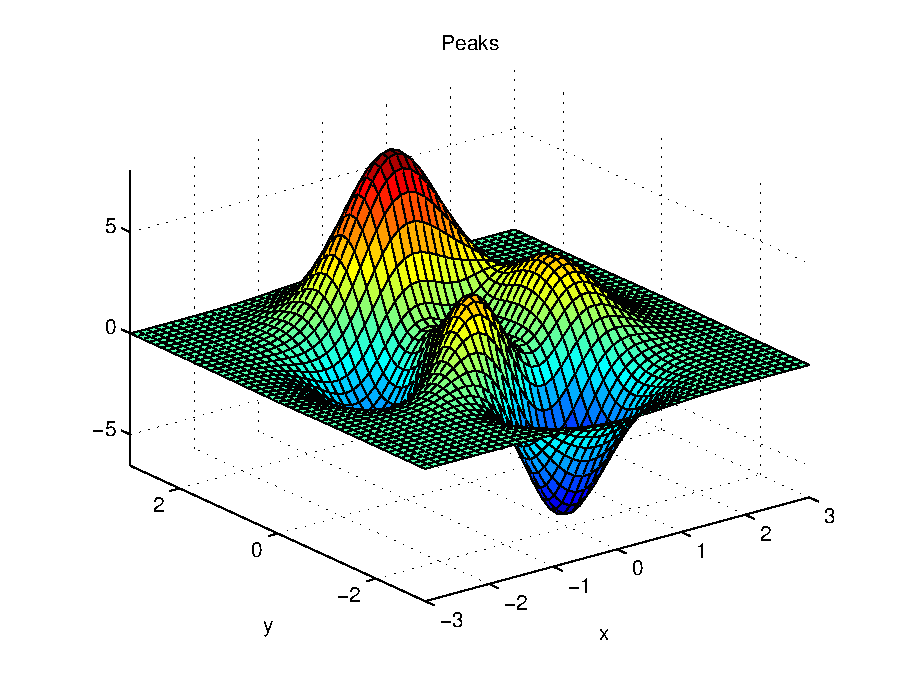
\includegraphics[width=12cm]{mcmthesis-aaa.eps}
%	\caption{aa} \label{fig:aa}
%\end{figure}





%\begin{equation}
%a^2 \label{aa1}
%\end{equation}
%about this eqref \eqref{aa1}

